%Template
% !TeX spellcheck = de 
\documentclass[a4paper]{scrartcl}
\usepackage[utf8]{inputenc}
%\usepackage[ngerman]{babel}
\usepackage{geometry,forloop,fancyhdr,fancybox,lastpage}
\usepackage{dsfont}
\usepackage{tikz}
\usepackage[utf8]{inputenc}
%\usepackage[T1]{fontec}
\usepackage{lmodern}
\usepackage{helvet}
\usepackage{geometry}
\usepackage{mathptmx}
\usepackage{amsmath}
\usepackage{amssymb}
\usepackage{graphicx}
\usepackage{tabularx}
\usepackage{ragged2e}
\usepackage{array}
\usepackage[ngerman]{babel}
%\usepackage[table,dvipsnames,svgnames]{xcolor}
\usepackage{lscape}

\usepackage{listings}
\lstset{frame=tb,
	language=Java,
	aboveskip=3mm,
	belowskip=3mm,
	showstringspaces=false,
	columns=flexible,
	basicstyle={\small\ttfamily},
	numbers=left,
	numberstyle=\tiny\color{gray},
	keywordstyle=\color{blue},
	commentstyle=\color{dkgreen},
	stringstyle=\color{mauve},
	breaklines=true,
	breakatwhitespace=true,
	tabsize=3
}
\geometry{a4paper,left=3cm, right=3cm, top=3cm, bottom=3cm}
% Diese Daten müssen pro Blatt angepasst werden:
\newcommand{\NUMBER}{6}
\newcommand{\EXERCISES}{3}
% Diese Daten müssen einmalig pro Vorlesung angepasst werden:
\newcommand{\COURSE}{Stochastik}
\newcommand{\TUTOR}{TBD}
\newcommand{\STUDENTA}{Stefan Wezel}
\newcommand{\STUDENTB}{Stefan Wezel}
\newcommand{\STUDENTC}{}
\newcommand{\DEADLINE}{07.06.2018}




%Math
\usepackage{amsmath,amssymb,tabularx}

%Figures
\usepackage{graphicx,tikz,color,float}
\graphicspath{ {home/stefan/picures/} }
\usetikzlibrary{shapes,trees}

%Algorithms
\usepackage[ruled,linesnumbered]{algorithm2e}

%Kopf- und Fußzeile
\pagestyle {fancy}
\fancyhead[L]{\STUDENTA}
\fancyhead[C]{\COURSE}
\fancyhead[R]{\today}

\fancyfoot[L]{}
\fancyfoot[C]{}
\fancyfoot[R]{Seite \thepage}

%Formatierung der Überschrift, hier nichts ändern
\def\header#1#2{
	\begin{center}
		{\Large\bf Übungsblatt #1}\\
		{(Abgabetermin #2)}
	\end{center}
}

%Definition der Punktetabelle, hier nichts ändern
\newcounter{punktelistectr}
\newcounter{punkte}
\newcommand{\punkteliste}[2]{%
	\setcounter{punkte}{#2}%
	\addtocounter{punkte}{-#1}%
	\stepcounter{punkte}%<-- also punkte = m-n+1 = Anzahl Spalten[1]
	\begin{center}%
		\begin{tabularx}{\linewidth}[]{@{}*{\thepunkte}{>{\centering\arraybackslash} X|}@{}>{\centering\arraybackslash}X}
			\forloop{punktelistectr}{#1}{\value{punktelistectr} < #2 } %
			{%
				\thepunktelistectr &
			}
			#2 &  $\Sigma$ \\
			\hline
			\forloop{punktelistectr}{#1}{\value{punktelistectr} < #2 } %
			{%
				&	
			} &\\
			\forloop{punktelistectr}{#1}{\value{punktelistectr} < #2 } %
			{%
				&
			} &\\
		\end{tabularx}
	\end{center}
}

\begin{document}

\section*{Aufgabe 23}
\subsection*{(a)}
Zunächst berechnen wir Durchschnitt und Varianz  eines 420 fachen Durchschnitt.\\
Erwartungswert:\\
$\mu = \sum_{i=1}^{420}E(X_i) = 420 \cdot E(X_1) = 420 \cdot 3.5 = 1470$
\\
\\
Varianz:\\
$\sigma = \sum_{i = 1}^{420} = 420 \cdot Var(X_1) = 420 \cdot \sqrt{\frac{35}{12}} = 717.29$
\\
\\
Nun berechnen wir den z-Wert:\\
$z = \frac{X_1 + .... + X_420-\mu}{\sigma} = \frac{1541-1470}{717.29} = \frac{71}{717.29} = 0.09$
\\
\\
Mithilfe einer Tabelle können wir nun: $F$ bestimmen.\\
$F(0.09) = 0.46414$

\subsection*{(b)}
Hier gehen wir ähnlich vor. Durchschnitt und Varianz können wir aus der letzten Teilaufgabe übernhemen.\\
Den z-Wert berechnen wir folgendermaßen:\\
$z = \frac{1436 - 1470}{717.29} = -0.48$\\
Jetzt betrachten wir wieder Tabelle:\\
$F(-0.48) = 0.31561$\\
Unsere Wahrscheinlichkeit beträgt: $1 - 0.31561 =0.68439$

\subsection*{(c)}
Durchschnitt und Varianz können wir wieder übernehmen.
Um die Wahrscheinlichkeit für das Intervall herauszufinden können wir die Wahrscheinlichkeit, dass die Augensumme kleiner 1469 von der Wahrscheinlichkeit dass die Augensumme kleiner als 1471 ist abziehen.\\
Wir berechnen also zuerst:\\
$z = \frac{1471 - 1470}{717.29} = \frac{1}{717.29} = 0.0014$\\
und dann:\\
$z = \frac{1469 - 1470}{717.29} = \frac{-1}{717.29} = -0.0014$\\
Eine Tabelle ist hier eher ungeeignet, also benutzen wir den R Befehl pnor(x) um die Wahrscheinlichkeit herauszufinden.\\
$F(0.0014) = 0.5005585$\\
und:\\
$F(-0.0014) = 0.4994415
$\\
Die Wahrscheinlichkeit, dass die Augensumme im gegebenen Intervall liegt ist:\\
$F(0.0014) - F(-0.0014) = 0.5005585 - 0.4994415 = 0.001117$


\subsection*{(d)}
Nach Satz 3.6 aus der Vorlesung gilt:\\
$P(Augensumme = 1470) = 0$, da es sich um eine absolut stetige Verteilungsfunktion handelt. 



\subsection*{Aufgabe 24}
\subsection*{(a)}
\begin{lstlisting}
x <- c(runif(1000000, min = 0, max = 1))
y <- c(runif(1000000, min = 0, max = 1))
z = x+y
\end{lstlisting}
\begin{figure}[H]
	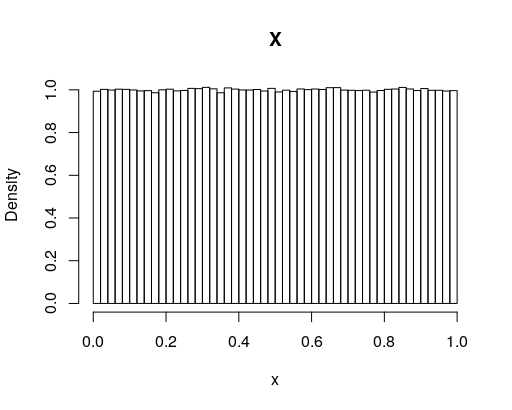
\includegraphics[scale=0.7]{Rplot02.png}
\end{figure}
\begin{figure}[H]
	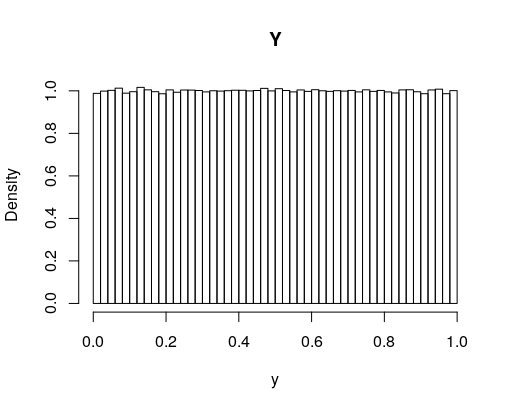
\includegraphics[scale=0.7]{Rplot03.png}
\end{figure}




\subsection*{(b)}
\begin{figure}[H]
	  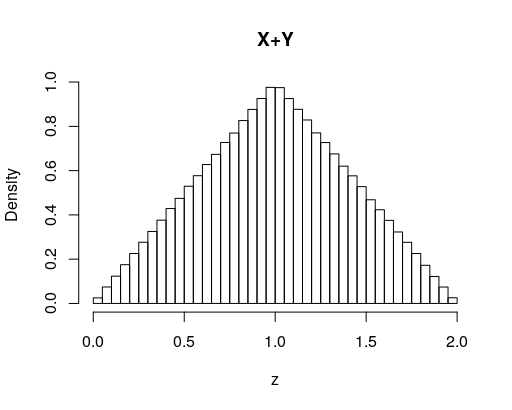
\includegraphics{Rplot01.png}
\end{figure}

\subsection*{(c)}
Die Verteilung nimmt die Form der Normalverteilung, also $P(x) = \frac{1}{{\sigma \sqrt {2\pi } }}e^{{{ - \left( {x - \mu } \right)^2 } \mathord{\left/ {\vphantom {{ - \left( {x - \mu } \right)^2 } {2\sigma ^2 }}} \right. \kern-\nulldelimiterspace} {2\sigma ^2 }}}$ an.






\subsection*{25}
\subsection*{(a)}
Wir können folgende Ungleichung aufstellen:\\

\begin{align*}
	\frac{100-400\cdot p}{\sqrt{400 \cdot p \cdot (p-1)}} &\leq F_{N(0,1)}^-1(0.7)\\\\
	\frac{100-400\cdot p}{\sqrt{400 \cdot p \cdot (p-1)}} &\leq 0.5244
\end{align*}
\end{document}
